In this section, we describe the workflow of the proposed methodology along with
the core ideas and models that the methodology is based on. Although our work is
closely related to simulation techniques, what we do is synthesis, not
simulation, which will become clear in the following subsections. An overview of
the methodology is depicted in \fref{methodology} and can be voiced as follows.
There are two major stages: data acquisition and data synthesis. The modules to
the left of the two clouds in \fref{methodology} correspond to the
data-acquisition stage, and the module to the right corresponds to the
data-synthesis state. The data-acquisition stage collects and stores reference
data while the data-synthesis stage fetches these data and produces power and
temperature traces of the system. There are two types of reference data: arrival
and workload, which are referred to as patterns in the figure and in what
follows. As the names suggest, the two pieces of information characterize job
arrivals and job workloads, and they will be further discussed in the following
two subsections, \sref{traffic} and \sref{workload}. In \sref{composition}, we
explain how the pieces are combined into a coherent whole.

\subsection{Arrivals} \slab{traffic}
\cite{leland1994}

In order to generate realistic steams of job arrivals, we have decided to use a
multifractal wavelet model \cite{riedi1999}, which was originally proposed in
the context of network traffic modeling. In vain with other studies
\cite{nikitovic2004}. We use a dataset published by Google \cite{google}. The
dataset contains usage data of a computational cluster over a month period (May
2011).


\subsection{Workloads} \slab{workload}
In the previous subsection, we introduced our approach to generating streams of
arrivals; however, an arrival is only a time stamp without any information about
the actual workload. In this subsection, we describe how workload candidates are
obtained and utilized for substantiating job arrivals, which is depicted at the
bottom of \fref{methodology}. To begin with, workload candidates should conform
to a number of criteria. First, since we aim to produce realistic trace,
workloads should represent well the applications or services that the system in
question is supposed to provide to the user. Second, a workload should be fast
to evaluate, which, in our context, refers to obtaining the power consumption
over time of that workload.

Our workload modeling is based on full-system simulations of reference programs.
However, if we had incorporated such simulations into our workflow
\emph{directly}, we would have wound up with a configuration similar to the one
displayed in \fref{development}. This, of course, would have defeated the
purpose of our work since, as motivated in \sref{motivation}, detailed
simulations are too time consuming. Instead, we propose the use of high-level
recordings; this functionality corresponds to the modules labeled ``Recorder''
in \fref{methodology}. To elaborate, using an adequate simulator capable of
modeling the target architecture, we execute each reference program in isolation
and record certain information about this execution.\footnote{Such a technique
is similar in spirit to PinPlay \cite{patil2010}, which is a tool for recording
and replaying an execution of a program at the instruction level.} At a later
stage of our pipeline (see the Streamer module in \fref{methodology}), the
collected information is utilized in order to flesh out jobs upon their arrival,
and this stage requires no simulation. These recordings are building blocks:
they are combined to form complex workloads corresponding to multiple programs
running in parallel, which will be elaborated on in \sref{composition}.

From our experience, performance and power simulation takes by far the largest
expense in terms of time. Therefore, the information about a reference program's
execution that we propose to record is the power consumption of that execution.
This approach pushes the aforementioned expense to the data-acquisition stage
and eliminates it all together from the data-synthesis stage. To put it
differently, each recording is obtained via a one-time simulation at the
data-acquisition stage, and from there on the recording is reused as many times
as needed at the data-synthesis stage of our methodology. Since the actual data
generation, which takes place at the data-synthesis stage, is deliver from the
expensive simulations, it has a very low computational demand. This demand is
negligible compared to the one of the scenario depicted in \fref{development},
in which one undertakes performance and power simulations nonstop.

The power consumption of a program can be recorded differently; let us be more
specific about what we do. The first aspect to note is that we record power as a
function of time (assuming a certain sampling interval). Second, the dynamic and
static components of the power consumption are recorded separately in order to
get a better control over the subsequent composition (\sref{composition}).
Third, the power consumption is recorded for all processing elements that are
relevant to the subsequent study (for instance, cores and shared caches).

The result of the recording procedure is a repository of power traces
corresponding to real programs, which we refer to as workload patterns; see the
bottom cloud in \fref{methodology}. Full-system simulations obviously take time;
however, as mentioned previously, they should be done only once. Moreover, since
researchers tend to test their ideas using similar sets of benchmark
suites---for example, \sc{PARSEC} \cite{bienia2011} and \sc{SPEC CPU2006}
\cite{cpu2006} are popular choices---it is reasonable to create a common
repository of power patterns that will be populated and maintained online by the
research community.

Let us now turn to the question: How do we choose which workload pattern to use
for a particular arrival? We shall refer to this functionality as the workload
model. The input to this model is a stream of arrival times, and its output is a
stream of fully characterized jobs (time and work). The logic of the workload
model can be dependent on the input stream and thereby introduce
autocorrelations to the output stream, which allows for modeling, for instance,
periodic and/or coupled workloads. Since such aspects rely heavily on
domain-specific knowledge, we refrain from providing any particular dependency
model. The default option that is used in our toolchain (to be discussed in
\sref{toolchain}) for assigning workloads to job arrivals is drawing samples
from a uniform distribution over a set of workload patterns. This default
behavior can be adjusted for the problem at hand as needed.

To recapitulate, we have obtained a database of reference workloads and
discussed the formation of job streams from arrival streams. The patterns
correspond to executions of real programs and, thus, exhibit realistic traits.


\subsection{Composition} \slab{composition}
\begin{figure}
  \centering
  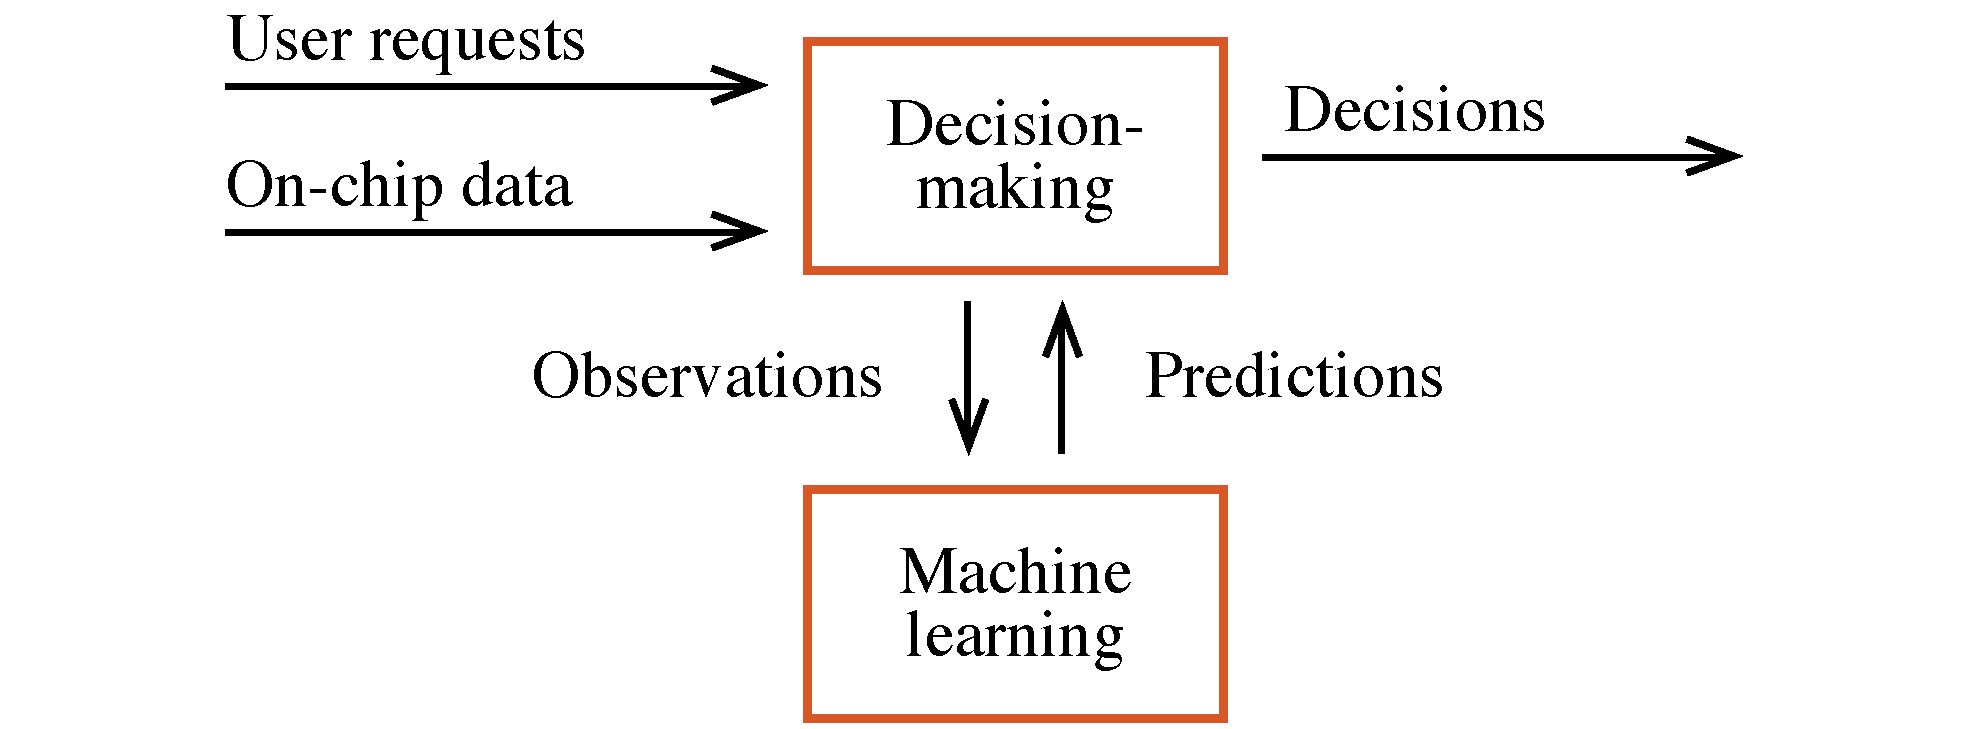
\includegraphics[width=1.0\columnwidth]{include/assets/figures/governor.pdf}

  \caption{A proactive governor of an electronic system. \emph{Observations}
  refers to the data used for learning. \emph{Predictions} refers to the data
  that the management strategy needs to know in advance in order to make
  proactive decisions.}

  \flab{governor}
\end{figure}

So far we have obtained two corresponding streams: arrival and workload. The two
streams merge into a new stream representing a sequence of concrete incoming
jobs or user requests, and this new stream needs to be processed, which is the
topic of this subsections. Here, \emph{processing} refers to progressively
building a schedule,\footnote{In this paper, mapping is assumed to be a part of
scheduling.} constructing a power profile, and computing the corresponding
temperature profile. In \fref{methodology}, this functionality resides in the
box labeled ``Streamer.''

As motivated in \sref{motivation}, a prominent use case of our methodology is
the development of management strategies. Therefore, the management core of the
system at hand is devised by the user, which is further detailed in
\sref{usage}. Hence, a scheduling policy is given, and it decides on a schedule.
Namely, each arrived job contains information about the computational resources
it needs, and the policy specifies when the job gets access to these resources.
Then we add accordingly the recorded (and potentially transformed) power pattern
of the job to the power profile of the system. A helpful analogy here might be
paving a road with rectangular bricks of different sizes. As the time goes by,
we feed the power profile to a temperature simulator and obtain a temperature
profile.

The power and temperature profiles are the final output of our methodology. The
key observation to be made is that no prohibitively expensive performance or
power simulations are involved in the data-synthesis stage. The time consumed by
the procedure delineated above is practically negligible.

At this point, we would like to draw attention to the following. It should be
clear that, by recording power directly, we make a trade-off, and making this
trade-off is necessary. Many details pertaining to programs' executions have
been discarded in order to gain speed. What has been baked into recordings
cannot be to altered at the data-synthesis stage in general. Consider, for
instance, a recording of a program that had two cores at its disposal. This
pattern cannot be used to replay the execution as if there was only one core.
Similarly, the recording cannot tell what would happen if the program could
leverage one additional core. Another limitation concerns resource sharing,
which is twofold. First, workload patterns obtained in isolation cannot used to
fabricate the interleaving of two programs (time sharing). Second, even if two
programs run on two different cores, they still can affect each other by
competing for such resources as shared L3 caches. Currently, the above concerns
can be addresses in our methodology only partially.


To summarize, the proposed methodology has been presented. The methodology is
composed of two stages. In the data-acquisition stage, reference arrival and
workload data are harvested. In the data-synthesis stage, the data are used to
generate a stream of jobs and subsequently compute a power and a temperature
profile. The produced data preserve the particularities of the reference data.
At the same time, the synthesis is fast as it bypasses expensive simulations.
